\chapter{Analisis Masalah Pengumpulan Data Pada \textit{Spreadsheet}}

Pada bab ini diuraikan analisis persoalan pengumpulan data pada \textit{spreadsheet} yang telah diuraikan pada Bab I. Hasil dari bab ini digunakan untuk merancang aplikasi yang akan diimplementasikan seperti yang dijelaskan pada Bab IV.

\section{Permasalahan Pengumpulan Data Pada \textit{Spreadsheet}} \label{AspekAplikasi}
Pada Subbab \ref{RumusanMasalah} telah dijelaskan bahwa terdapat tiga permasalahan yang muncul didalam pengumpulan data menggunakan media \textit{spreadsheet} yakni:
\begin{enumerate}
	\item Kolaborasi \\
	Didalam pembuatan suatu \textit{spreadsheet}, kadang dibutuhkan banyak pihak untuk dapat melengkapi seluruh data yang dibutuhkan. Hal ini membuat pengembangan dan pengumpulan data membutuhkan kontribusi banyak orang \citep{Panko1998}. Untuk itu dibutuhkan fitur kolaborasi pada aplikasi \textit{spreadsheet} agar banyak pihak dapat melakukan pengumpulan data dan pengeditan secara bersamaan.
	\item Validasi \\
	Data yang dikumpulkan pada suatu \textit{spreadsheet}, sangat rentan akan kesalahan. Bahkan pada \textit{spreadsheet} yang dibuat dengan sangat hati-hati, masih dapat ditemui sekitar 1 persen atau lebih kesalahan pada formula yang dibuat \citep{Panko1998}. Sehingga dibutuhkan mekanisme tambahan pada saat pengumpulan data untuk melakukan validasi terhadap masukan.
	\item Penyimpanan Data \\
	Setelah data dikumpulkan, permasalahan selanjutnya yang muncul adalah penyimpanan data tersebut. Data biasanya akan tetap tersimpan dalam bentuk berkas \textit{spreadsheet}, namun bentuk ini sulit untuk digunakan oleh aplikasi lain. Bentuk yang biasanya digunakan oleh aplikasi lain untuk dapat mengambil dan menyimpan data adalah bentuk relasional. Sehingga dibutuhkan mekanisme penyimpanan data ke dalam bentuk relasional agar data dapat dengan mudah digunakan pada aplikasi lain.
\end{enumerate}

Ketiga permasalahan tersebut yang dijadikan dasar pengembangan aplikasi pada Tugas Akhir ini. Aplikasi yang dibuat akan mengubah alur penggunaan \textit{spreadsheet} yang umum dengan menambahkan mekanisme-mekanisme yang dibutuhkan. Alur aplikasi yang lama dapat dilihat pada Gambar \ref{GambarWorkflowBiasa} dan aplikasi \textit{spreadsheet} yang dibangun pada Tugas Akhir ini pada Gambar \ref{GambarWorkflow}.

	\begin{figure}[htb]
	    \centering
	    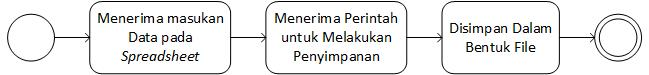
\includegraphics[width=0.7\textwidth]{resources/chapter-3-workflow-biasa.jpg}
	    \caption{Alur Kerja Aplikasi \textit{Spreadsheet} Biasa}
		\label{GambarWorkflowBiasa}
	\end{figure}

	\begin{figure}[htb]
	    \centering
	    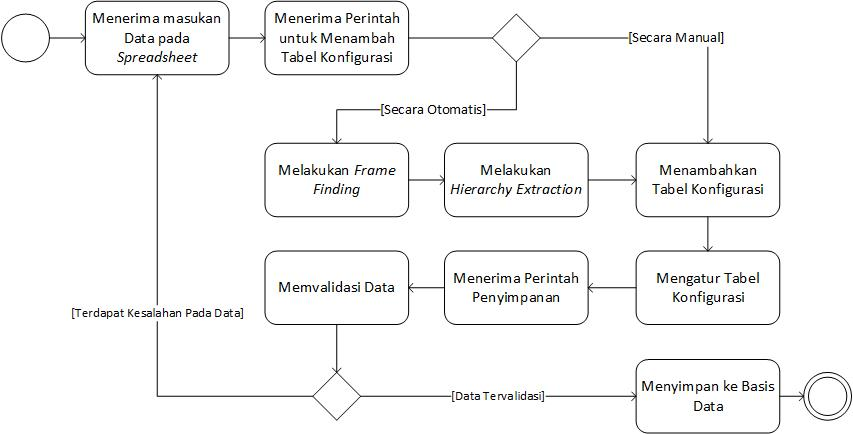
\includegraphics[width=1\textwidth]{resources/chapter-3-workflow.jpg}
	    \caption{Alur Kerja Aplikasi \textit{Spreadsheet} yang Akan Dibuat}
		\label{GambarWorkflow}
	\end{figure}

Dapat dilihat bahwa terdapat proses tambahan yang dilakukan pada aplikasi yang akan dibuat. Proses tersebut terdiri dari pencarian bagian label dan data serta proses validasi. Hasil dari identifikasi label dan data akan dijadikan \textit{tuple} relasional yang disimpan dalam bentuk basis data. Alur kolaborasi bukan merupakan fokus pengembangan Tugas Akhir ini sehingga akan ditangani oleh aplikasi \textit{spreadsheet} yang dipilih.

% Pada Subbab \ref{KesalahanPenggunaan} dijelaskan bahwa terdapat dua jenis kesalahan yang dapat terjadi pada penggunaan \textit{spreadsheet} yakni kesalahan kualitatif dan kesalahan kuantitatif. Kesalahan kualitatif merupakan kesalahan penggunaan \textit{spreadsheet} yang berhubungan dengan kualitas dan prosedur penggunaan. Contoh kesalahan kualitatif yang sering terjadi adalah penggunaan \textit{spreadsheet} sebagai basis data. Kesalahan kuantitatif merupakan kesalahan yang menyebabkan keluaran menjadi salah. Contoh kesalahan kuantitatif yang sering terjadi adalah kesalahan masukan yang tidak divalidasi.

% Pencegahan untuk kesalahan-kesalahan ini dapat dilihat pada Subbab \ref{PenangananKesalahan}. Salah satu caranya adalah pembuatan \textit{preliminary design} terhadap \textit{spreadsheet} yang dibuat. Hal ini dapat dilakukan dengan cara pengembangan aplikasi pengumpulan data berbentuk \textit{spreadsheet} yang menangani kolaborasi, validasi, dan penyimpanan. Dengan aplikasi ini diharapkan dapat menangani kesalahan kualitatif seperti yang dijelaskan pada contoh sebelumnya yakni penggunaan \textit{spreadsheet} sebagai basis data dengan cara menghubungkan \textit{spreadsheet} ke basis data yang sesungguhnya secara langsung. Serta menangani kesalahan kuantitatif dengan cara melakukan validasi masukan.

% Aplikasi \textit{spreadsheet} yang baik harus dapat diakses dan digunakan secara kolaboratif yang dapat dilakukan dengan membuat aplikasi \textit{spreadsheet} tersebut berbasis \textit{web}. Aspek-aspek aplikasi \textit{web} yang perlu diperhatikan dalam membangun aplikasi \textit{spreadsheet} adalah:
% \begin{enumerate}
% 	\item \textit{Response time}\\
% 	Membangun aplikasi berbasis \textit{web} menggunakan HTTP sebagai protokol komunikasi dan tentunya didalam komunikasi tersebut membutuhkan waktu untuk mengirimkan \textit{request} dari klien. Jika waktu yang dibutuhkan untuk melakukan respon lambat, akan sulit terjadi kolaborasi dan memperbesar kemungkinan terjadinya \textit{race condition} pada masukan pengguna. Sehingga diperlukan waktu respon yang cepat untuk dapat menangani banyak \textit{request} dalam satu waktu dan dalam waktu yang singkat.

% 	\item Akses yang konkuren\\
% 	Aplikasi berbasis \textit{web} yang akan dibuat harus dapat diakses secara konkuren yakni diakses bersama-sama oleh banyak klien dalam satu waktu. Pengaksesan secara konkuren dapat berdampak pada terpanggilnya banyak \textit{query} dalam satu waktu. Oleh karena itu aplikasi yang dibuat harus dapat menjalankan secara konkuren setiap \textit{request} yang masuk.

% 	\item Akses basis data\\
% 	Akses terhadap basis data dibutuhkan sebagai media penyimpanan yang persisten dan konsisten. Oleh karena itu, akses terhadap basis data diperlukan untuk kemudahan penyimpanan dan pengambilan data serta mengatasi permasahalan ketidaksamaan \textit{versioning} diantara suatu \textit{file spreadsheet}.

% \end{enumerate}

% Keempat aspek pada aplikasi berbasis \textit{web} tersebut akan menjadi aspek utama yang dikembangkan didalam pembuatan aplikasi \textit{spreadsheet} berbasis aplikasi \textit{web}.

% Berdasarkan pada Subbab \ref{KesalahanPenggunaan}, terdapat dua jenis tipe kesalahan \citep{Panko1998} yang bisa terjadi pada penggunaan \textit{spreadsheet} yakni:
% \begin{enumerate}
% 	\item Kesalahan Kualitatif

% 	Kesalahan kualitatif merupakan kesalahan yang berhubungan dengan kualitas yang dipengaruhi oleh prosedur pembuatan dan rancangan pada \textit{spreadsheet} tersebut. Contoh kesalahan kualitatif yang sering terjadi adalah penggunan \textit{spreadsheet} sebagai media penyimpanan atau basis data. Hal ini tidak sesuai dengan kegunaan utama dari \textit{spreadsheet} sebagai media kalkulasi dan perhitungan statistik.

% 	\item Kesalahan Kuantitatif

% 	Kesalahan kuantitatif merupakan kesalahan yang menyebabkan hasil perhitungan menjadi salah atau tidak valid. Contoh kesalahan jenis ini yang sering terjadi adalah kesalahan mekanikal dimana pengguna salah memasukan data yang tidak sesuai dengan konstrain yang ada. Hal ini dapat diatasi dengan adanya validasi sebelum data diterima. 
% \end{enumerate}

% Dari kedua tipe tersebut, pada Tugas Akhir ini akan lebih ditekankan kepada kesalahan kuantitatif yang bertipe kesalahan mekanikal dengan memanfaatkan teknik validasi pada masukan. 

% Dengan menggunakan aplikasi ini, terdapat perubahan alur penggunaan \textit{spreadsheet}. Gambar dibawah ini merupakan alur penggunaan aplikasi \textit{spreadsheet} biasa pada Gambar \ref{GambarWorkflowBiasa} dan aplikasi \textit{spreadsheet} yang dibangun pada Tugas Akhir ini pada Gambar \ref{GambarWorkflow}. 

% 	\begin{figure}[htb]
% 	    \centering
% 	    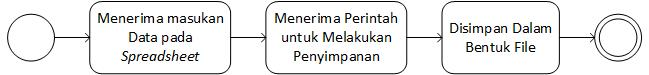
\includegraphics[width=0.7\textwidth]{resources/chapter-3-workflow-biasa.jpg}
% 	    \caption{Alur Kerja Aplikasi \textit{Spreadsheet} Biasa}
% 		\label{GambarWorkflowBiasa}
% 	\end{figure}

% 	\begin{figure}[htb]
% 	    \centering
% 	    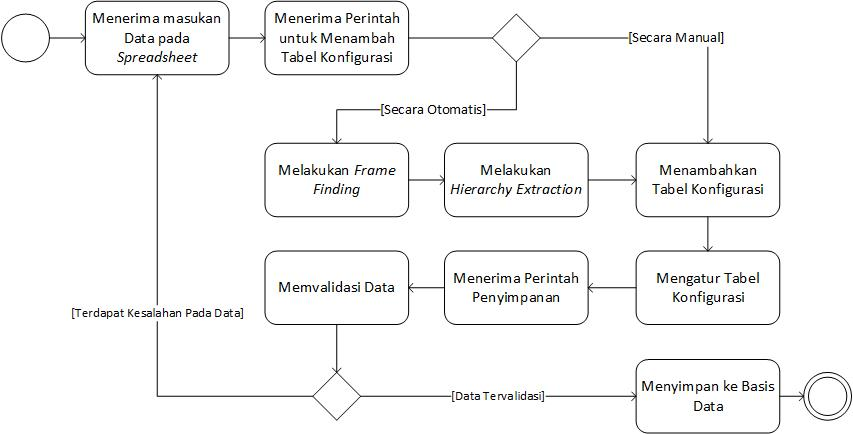
\includegraphics[width=1\textwidth]{resources/chapter-3-workflow.jpg}
% 	    \caption{Alur Kerja Aplikasi \textit{Spreadsheet} yang Akan Dibuat}
% 		\label{GambarWorkflow}
% 	\end{figure}

% Dapat dilihat bahwa terdapat proses tambahan yang dilakukan pada aplikasi yang akan dibuat. Proses tersebut terdiri dari pencarian bagian label dan data serta proses validasi. Hasil dari identifikasi label dan data akan dijadikan \textit{tuple} relasional yang disimpan dalam bentuk basis data.

\section{Analisis Rancangan Aplikasi \textit{Spreadsheet}}
Dari permasalahan yang telah didefinisikan pada subbab \ref{AspekAplikasi}, dapat ditentukan beberapa hal yang harus dianalisis dalam merancang aplikasi \textit{spreadsheet} ini, diantaranya adalah:
\begin{enumerate}
	\item Penentuan aplikasi \textit{spreadsheet} yang akan dikembangkan dan ditambahkan fiturnya. Aplikasi harus memiliki fitur kolaborasi sehingga banyak pengguna dapat mengakses suatu \textit{spreadsheet} secara bersamaan.  
	\item Pemilihan model interaksi aplikasi \textit{spreadsheet} dimana pengguna dapat membentuk struktur tempat pengguna lain memasukan input. Contohnya dalam bentuk tabel atau formulir. Pengguna juga melengkapi domain dan batasan data yang dimasukkan.
	\item Setelah pengguna selesai merancang struktur masukan, diperlukan penentuan bagian label dan data yang berkaitan dengan label tersebut. Bagian label dan data akan dijadikan menjadi bentuk relasional yang dapat disimpan dalam basis data
	\item Pengguna lain yang hanya memiliki kapabilitas pengisian data, hanya dapat mengisi data sesuai struktur yang diberikan. Sehingga perlu melakukan validasi data dan dicek kesesuaiannya sesuai dengan batasan yang diberikan sehingga memenuhi domain yang ditentukan pada basis data.
	\item Setelah proses validasi terpenuhi, diperlukan cara penyimpanan data sesuai dengan relasi \textit{tuple} yang telah ditentukan. Pada saat pembukaan \textit{file spreadsheet} tersebut, akan dilakukan pemulihan data yang telah disimpan pada basis data untuk ditampilkan kembali.
\end{enumerate}
Pada subbab-subbab selanjutnya, akan dibahas analisis untuk kelima poin diatas yang selanjutnya akan dijadikan dasar rancangan fitur yang akan dibuat pada aplikasi \textit{spreadsheet}.

\section{Analisis Perbandingan Aplikasi \textit{Spreadsheet} yang Dikembangkan}
Dari studi yang telah dilaksanakan pada subbab \ref{TeknologiSpreadsheet}, aplikasi \textit{spreadsheet} dapat dibagi berdasarkan konektivitasnya yakni \textit{offline spreadsheet} dan \textit{online spreadsheet} dan dapat juga dibagi lagi berdasarkan keterbukaan dari \textit{source code} yakni \textit{open source} dan \textit{closed source}. Pada Tabel \ref{AnalisisAplikasiDasar} dijabarkan parameter yang mendasari pemilihan aplikasi yang akan dikembangkan.

\begin{longtable}{ | p{3cm} | p{4cm} | p{4cm} | }
    \caption{Perbandingan Aplikasi \textit{Spreadsheet}}
    \label{AnalisisAplikasiDasar}\\ \hline
    \centering\bfseries{Parameter} & \centering\bfseries{Offline Application} & \centering\bfseries{Web/Online Application} \tabularnewline \hline
    \endfirsthead
    \hline
    \centering\bfseries{v} & \centering\bfseries{Manual oleh Pengguna} & \centering\bfseries{Otomatis} \tabularnewline \hline
    \endhead
    Aksesibilitas & Dibutuhkan instalasi aplikasi / plugin yang bersangkutan. & Dapat menggunakan web browser yang tersedia. \\ \hline
    Kolaborasi & Tidak tersedia secara online dan kolaboratif secara \textit{default}. & Secara \textit{default}, dapat diakses konkuren dan kolaboratif. \\ \hline
    Fitur & Sudah banyak jenis formula yang didukung. & Tidak semua formula yang ada didukung. \\ \hline
\end{longtable}

Dari perbandingan diatas, diambil solusi dengan menggunakan aplikasi \textit{spreadsheet} berbasis web yang dapat diakses secara konkuren dan memiliki \textit{portability} yang lebih baik. Selain itu, untuk dapat mengembangkan fitur aplikasi dengan lebih baik, akan dipilih aplikasi yang berbentuk \textit{open source}. Sehingga dipilih aplikasi yang memiliki tipe \textit{online spreadsheet} dan \textit{open source} yaitu EtherCalc. Fitur kolaborasi yang dibutuhkan akan ditangani oleh aplikasi EtherCalc ini dan bukan merupakan bagian dari fitur yang akan dikembangkan.

\section{Analisis Model Interaksi Pengguna}
Di dalam pembangunan perangkat lunak \textit{spreadsheet} untuk mengurangi kesalahan, dapat diidentifikasikan dua model interaksi yang dapat diimplementasi. Model interaksi yang pertama adalah menggunakan formulir sebagai basis masukan data dan model yang kedua adalah menggunakan aplikasi \textit{spreadsheet} secara langsung sebagai media input data.
	\subsection{Berbasis Formulir}
	Model interaksi ini menggunakan \textit{spreadsheet} sebagai tempat perancangan formulir. Pembuat formulir akan menentukan area label dan input secara manual serta diidentifikasikan berdasarkan warna atau properti lain yang unik pada sel tersebut. Formulir akan dibangkitkan oleh aplikasi agar menjadi bentuk HTML dan terhubung ke basis data. Pengisian data oleh pengguna dilakukan melalui formulir yang dibangkitkan dan dapat diakses melalui web. Beberapa cara dapat dilakukan untuk mengimplementasikan teknik ini antara lain, mengembangkan dari aplikasi \textit{spreadsheet} yang telah ada menggunakan \textit{plugin} atau membuat aplikasi baru yang dapat melakukan konversi otomatis menjadi formulir.

	\subsection{Berbasis \textit{Spreadsheet}}
	Model interaksi berbasiskan \textit{spreadsheet} menggunakan antarmuka yang telah disediakan oleh aplikasi. Penggunaannya dilakukan dengan membuat format pengisian seperti membuat tabel pada \textit{spreadsheet} pada umumnya. Pada tabel harus terdapat label dan data sehingga metadata minimal yang dibutuhkan dapat dicapai. Fitur-fitur yang ada pada \textit{spreadsheet} juga tetap dapat digunakan saat pembuatan tabel yang diinginkan. Dari pembuatan tabel tersebut dilakukan identifikasi label dari data tersebut untuk selanjutnya diproses melalui penyaringan masukan dan dimasukan ke tabel yang sesuai yang ada di basis data. Untuk mengimplementasikan teknik ini harus mengubah kode pada program \textit{spreadsheet} atau mengekstensi fitur yang ada menggunakan \textit{plugin}. 

	\subsection{Perbandingan Model Interaksi}
	Kedua model interaksi tersebut memiliki beberapa perbedaan dan efek terhadap penggunaannya baik bagi sistem maupun pengguna. Pada Tabel \ref{ModelInteraksi} dijabarkan perbandingan antara kedua model interaksi tersebut.

	\begin{longtable}{ | p{3cm} | p{4cm} | p{4cm} | }
	    \caption{Perbandingan Model Interaksi}
	    \label{ModelInteraksi}\\ \hline
	    \centering\bfseries{Parameter} & \centering\bfseries{Berbasis Formulir} & \centering\bfseries{Berbasis \textit{Spreadsheet}} \tabularnewline \hline
	    \endfirsthead
	    \hline
	    \centering\bfseries{Parameter} & \centering\bfseries{Berbasis Formulir} & \centering\bfseries{Berbasis \textit{Spreadsheet}} \tabularnewline \hline
	    \endhead
	    Fungsionalitas & Berhasil memisahkan bagian operasional dan data. Pengguna hanya memodifikasi dan melakukan input pada bagian data. Bagian operasional hanya dapat dimodifikasi oleh pembuat formulir tersebut. & Jika tidak menggunakan proteksi terhadap sel yang dapat ditulis, tidak terjadi pemisahan antara data dan operasional sehingga beberapa kesalahan yang terjadi pada saat input masih dapat terjadi. \\ \hline
	    Teknologi & Dibutuhkan adanya algoritma tambahan untuk menangani formulir dan masukannya, serta melakukan konversi dan \textit{parsing} dari sel pada \textit{spreadsheet} ke dalam bentuk formulir. & Dibutuhkan algoritma dan logika \textit{parsing} yang lebih detil dan kompleks dalam menangani kasus-kasus table tertentu. \\ \hline
	    Antarmuka & Menggunakan antarmuka formulir yang kaku terurut dari atas ke bawah serta tidak dapat melihat hasil masukan secara langsung. & Struktur tabel atau masukan dapat disesuaikan dengan kebutuhan dan tidak perlu mempelajari hal lain jika sebelumnya telah menggunakan \textit{spreadsheet} sebagai media untuk memasukan data. \\ \hline
  	\end{longtable}

  	Pada Tugas Akhir ini, akan dipilih model interaksi dengan berbasis \textit{spreadsheet} sehingga pengguna dapat dengan lebih mudah didalam menggunakannya karena tidak memerlukan pembelajaran kembali di dalam menggunakan aplikasi. Selain itu, data yang dimasukan lebih mudah untuk dilihat secara menyeluruh dibandingkan dengan berbasis formulir yang hanya dapat menerima satu masukan dalam suatu formulir.

\section{Analisis Penentuan Bagian Data dan Label}
Pada pembuatan \textit{spreadsheet} pada umumnya, didapatkan bahwa kebanyakan \textit{spreadsheet} pada umumnya berbentuk tabel yang terdiri dari dua unsur utama yakni data dan label atau disebut juga tipe \textit{data frame} \citep{Chen2013}. Bagian data merupakan bagian yang biasanya dinamis dan merupakan masukan pengguna. Bagian label merupakan bagian yang memberikan keterangan dan konteks mengenai data yang dimaksud. Pada Gambar \ref{DataFrameSederhana} dapat dilihat bahwa area dengan nomor 1 disebut sebagai label yang menjelaskan data-data dibawahnya yakni pada area nomor 2.

\begin{figure}[htb]
    \centering
    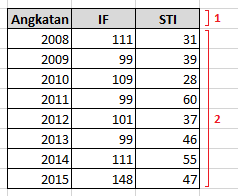
\includegraphics[width=0.3\textwidth]{resources/chapter-3-simple-dataframe.png}
    \caption{Contoh \textit{Data Frame} Sederhana}
	\label{DataFrameSederhana}
\end{figure}

	\subsection{Secara Manual}
	Penentuan label dan data dilakukan oleh pengguna secara langsung saat pembuatan tabel. Pengguna sendiri yang menentukan area mana yang merupakan label dan data mana yang dijelaskan oleh label tersebut. Dengan metode manual ini, pengguna dapat menyesuaikan bentuk tabel sesuai keinginan mereka. Metode ini menyerahkan sepenuhnya tanggungjawab keterhubungan sel label dan sel data kepada pengguna.

	\subsection{Secara Otomatis}
	Pencarian label dan data dapat menggunakan algoritma seperti yang telah dijelaskan pada Subbab \ref{metodepencarian}. Mekanisme untuk mengidentifikasi label dan data dapat dilakukan melalui 3 tahapan yakni, \textit{frame finder}, \textit{hierarchy extractor}, dan \textit{tuple builder}. Pada tahap pertama yakni \textit{frame finder} bertujuan untuk mengidentifikasi wilayah nilai (data) dan wilayah atribut (label) yang dapat berupa \textit{left attribute} maupun \textit{top attribute}. Tahap selanjutnya adalah \textit{hierarchy extractor} bertujuan untuk mendapatkan hirarki dari atribut-atribut yang ada sehingga label yang tertulis dapat dicari keterhubungan dan konteksnya terhadap data yang ada. Tahap terakhir adalah \textit{tuple builder} yang mentrasformasikan data dan label tersebut dalam bentuk \textit{tuple} yang dapat diterima oleh basis data relasional.

	\subsection{Perbandingan Metode Penentuan}
	Untuk mengetahui perbandingan kedua metode, pada Tabel \ref{MetodePenentuan} dijelaskan kelebihan dan kekurangan dua metode yang telah disebutkan sebelumnya.
	\begin{longtable}{ | p{3cm} | p{4cm} | p{4cm} | }
	    \caption{Perbandingan Metode Penentuan Data dan Label}
	    \label{MetodePenentuan}\\ \hline
	    \centering\bfseries{Keterangan} & \centering\bfseries{Manual oleh Pengguna} & \centering\bfseries{Otomatis} \tabularnewline \hline
	    \endfirsthead
	    \hline
	    \centering\bfseries{Keterangan} & \centering\bfseries{Manual oleh Pengguna} & \centering\bfseries{Otomatis} \tabularnewline \hline
	    \endhead
	    Kelebihan & Tingkat akurasi lebih tinggi karena data dan label yang ditentukan sesuai dengan keinginan pengguna. & Kenyamanan dalam penggunaan karena pengguna tidak perlu melakukan interferensi tambahan. Selain itu, sistem kemungkinan data dan label yang diambil dapat diubah ke dalam bentuk \textit{tuple} relasional lebih tinggi. \\ \hline
	    Kekurangan & Interferensi pengguna yang banyak dan mungkinnya data dan label tidak dapat dijadikan bentuk \textit{tuple} relasional. & Algoritma ini hanya optimal jika digunakan pada tabel yang terurut vertikal. \\ \hline
  	\end{longtable}
  	Dari perbandingan diatas, dapat dilihat terdapat kekurangan dan kelebihan didalam menggunakan salah satu metode tersebut. Berdasarkan hal tersebut, yang akan dipilih sebagai metode penentuan data dan label adalah gabungan dari kedua metode tersebut. Sistem awalnya akan melakukan \textit{parsing} terhadap struktur yang telah dibuat oleh pengguna, kemudian pengguna dapat melihat hasil dari \textit{parsing} tersebut sehingga pengguna dapat memperbaiki jika terdapat hasil pelabelan yang salah. Dengan metode gabungan ini diharapkan dapat meningkatkan akurasi dan mengurangi kesalahan \textit{parsing} yang terjadi namun tetap memberikan kenyamanan terhadap pengguna serta menjaga agar hasil pelabelan tetap dapat diubah ke dalam bentuk \textit{tuple} relasional.

\section{Analisis Validasi Data}
Setelah pengguna memasukan datanya kedalam struktur yang telah ditetapkan, pengecekan data dilakukan. Tujuan dari mekanisme ini adalah untuk menghindari kesalahan masukan yang terjadi dan menyesuaikan tipe yang diterima oleh tabel pada basis data. Terdapat tiga hal utama yang divalidasi pada aplikasi ini, yakni:
\begin{enumerate}
	\item Validasi tipe data. Contohnya, data masukan yang seharusnya berupa \textit{integer} tidak dapat menerima masukan berupa \textit{string}.
	\item Validasi domain masukan. Pengguna dapat juga mengatur rentang \textit{integer} yang boleh dijadikan masukan atau \textit{string} apa saja yang dapat diterima oleh sistem.
	\item Validasi relasi data. Data masukan dapat berupa nilai yang harus ada pada tabel lain, contohnya terdapat 2 tabel yakni nilai mahasiswa dan identitas mahasiswa. Tabel nilai mahasiswa memiliki kolom NIM yang nilainya harus ada pada tabel identitas mahasiswa. Pada \textit{spreadsheet} biasanya hal ini diatasi dengan menggunakan perintah VLOOKUP.
\end{enumerate}
Sistem akan melakukan validasi terhadap ketiga hal tersebut dan menolak data masukan sehingga pengguna dapat memperbaiki data. 

\section{Penyimpanan Data}
Data yang telah dimasukan oleh pengguna baik data bentuk struktur \textit{spreadsheet} maupun data masukan pada struktur disimpan ke dalam basis data yang presisten. Terdapat 2 jenis data yang harus disimpan ke dalam basis data di dalam membangun aplikasi \textit{spreadsheet} ini, yakni:

\begin{enumerate}
	\item Penyimpanan \textit{File Spreadsheet} \\
	\textit{File spreadsheet} yang dimaksud adalah data struktural seperti \textit{value} pada suatu sel, \textit{properties} suatu sel seperti warna, \textit{border}, dan \textit{alignment}, serta hal-hal lain yang berhubungan dengan bagaimana suatu \textit{file spreadsheet} ditampilkan pada aplikasi. Tipe penyimpanan yang dapat digunakan untuk menampung data ini adalah NoSQL karena tipe ini cocok untuk menangani data yang kurang terstruktur seperti \textit{file spreadsheet} yang struktur penempatan datanya berbeda tiap pengguna. Cara penyimpanan yang cocok untuk menangani struktur ini adalah \textit{document based} atau \textit{key-value}.

	\item Penyimpanan Data dan Label \\
	Data yang disimpan merupakan hasil dari pendeteksian label dan data yang akan diubah menjadi \textit{tuple} relasional yang dapat diterima oleh basis data relasional. Contoh pengubahan yang terjadi dapat dilihat pada Gambar \ref{RelationalTuple}.

	\begin{figure}[htb]
	    \centering
	    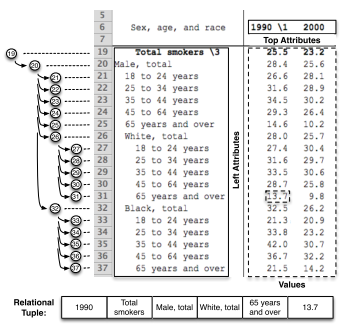
\includegraphics[width=0.6\textwidth]{resources/chapter-3-relational-tuple.png}
	    \caption{Contoh \textit{Tuple} Relasional}
		\label{RelationalTuple}
	\end{figure}

	Setelah data dan label dijadikan \textit{tuple} relasional, \textit{tuple} dimasukan ke dalam basis data dengan menggunakan operasi \textit{insert} ke dalam tabel pada basis data. Tipe penyimpanan yang cocok digunakan adalah basis data relasional (SQL) karena data yang dibuat dalam bentuk tabel pada umumnya dapat dikonversikan menjadi \textit{tuple} relasional.
\end{enumerate}

% \section{Rencana Tindak Lanjut}
% Berdasarkan analisa yang telah dijelaskan pada bab-bab sebelumnya, pada Tugas Akhir ini akan dibangun aplikasi \textit{spreadsheet} dengan menggunakan EtherCalc sebagai teknologi utama. Pada Subbab \ref{TeknologiSpreadsheet} telah dijelaskan bahwa EtherCalc merupakan perangkat lunak \textit{spreadsheet} yang \textit{open source} dan memiliki kemampuan kolaborasi didalam penggunaannya. Sehingga dengan menggunakan EtherCalc, aspek-aspek yang telah dijelaskan pada Subbab \ref{AspekAplikasi} yang harus ada didalam pembangunan \textit{spreadsheet} ini sudah dapat dipenuhi. Pada Tugas Akhir ini akan dilakukan pengembangan dari EtherCalc yang berupa identifikasi label dan data, penanganan validasi data dan keterhubungannya dengan basis data relasional. Alur kerja dari aplikasi \textit{spreadsheet} yang akan dibuat dapat dilihat pada Gambar \ref{GambarWorkflow} pada Subbab \ref{AspekAplikasi}.